\section{Enumeratoren und Konfiguration von Test}

Die Konfiguration eines Test wird von der Klasse \texttt{Executor} vorgenommen. Iteriert über die Liste der Konfigurationsobjekte, die mit dem \texttt{Configurator} erzeugt wurden. Für jede Regelmenge, die in einem Test festgelegt ist, wird ein eigener initaler Plan erzeugt. Der Enumerator wird mit einer Regelmenge initalisiert. Jetzt kann die Zeitmessung gestartet werden und der initale Plan an den Enumerator übergeben werden. Der Enumerator führt die Regeln aus. Das Ergebnis ist eine expandierte Äquivalenzklasse. Die an die Kostenschätzung weitergegeben wird. Ist hier der optimale Plan ermittelt, stoppt die Zeit und die Messung kann gespeichert werden.



\begin{figure}[ht]
  \centering
  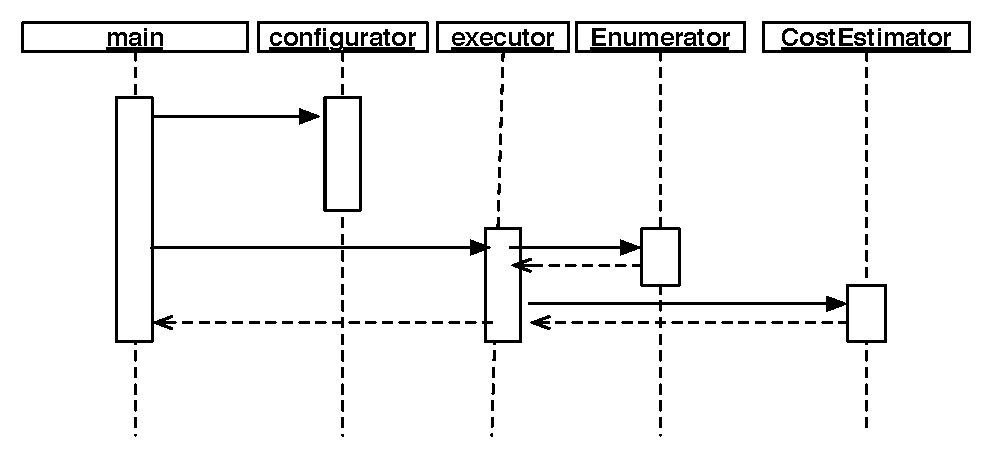
\includegraphics[width=\textwidth]{04_Implementierung/00_media/SequenceDiagramConfiguration.pdf}
  \caption{Sequenzdiagramm: Aufruf von Main zu Enumerator}
  \label{SequenceDiagramConfiguration}
\end{figure}
